\documentclass[11pt]{amsart}

% Standard letter size paper with 1inch margins
\usepackage[letterpaper, margin=1in]{geometry}

% Useful packages 
\usepackage{amsmath, amssymb, amsthm, amsaddr}
\usepackage{enumerate, subcaption, graphicx, hyperref}
\usepackage{algorithm}
\usepackage{algpseudocode}
\usepackage{cite}

\newcommand{\I}{\mathrm{i}}
\DeclareMathOperator{\E}{e}

\title{AMATH 582: Homework 2}
\author{Hunter Lybbert} % first and last name

\address{Applied Mathematics Department, University of Washington, Seattle, WA 
\\ \texttt{hlybbert@uw.edu}}

\date{\today} % you can also just type the date instead of "\today"

\begin{document}

\maketitle

\begin{abstract}
    In this analysis of the joint movement data of OptimuS-VD we experiment with Principal Component Analysis (PCA) as a means of dimensionality reduction.
    Our goal was to build a projection of the recordings to a lower dimension than the number of coordinates, visualize the movements in this new lower dimension.
    Using the lower dimensional projection we design an algorithm that recognizes which movement OptimuS-VD is performing.
    Furthermore, we first implemented a clustering-esque classifier and evaluate it's accuracy using the training set as well as the held out test set.
    Considerations of further work are given.
\end{abstract}

\section{Introduction and Overview}\label{sec:Introduction}
There are many computationally intensive computer vision models (primarily using convolutional neural-networks) that perform well on object and movement recognition.
This was all kickstarted by a paper published in \textit{Advances in Neural Information Processing Systems} by Krizhevsky et. al.  \cite{NIPS2012_c399862d}.
In our analysis we do not make use of neural networks or deep learning, we will primarily use the Singular Value Decomposition (SVD) via PCA.
In order to understand the data and attempt to classify the movements of the robot we aimed to complete the following 5 tasks: \\
\begin{enumerate}

\item Perform PCA on our robot movement data such that PCA modes are spatial modes and coefficients are time-dependent coefficients.
Investigate how many PCA spatial modes you need to keep to approximate $X_{\rm Train}$ up to 70\%, 80\% , 90\% , 95\% in Frobenius norm (i.e., energy) and plot results. \\

\item Truncate the PCA modes set to 2 and 3 modes and plot the projected $X_{\rm Train}$ in the truncated PCA space as low dimensional 2D (PC1,PC2 coordinates) and 3D (PC1,PC2,PC3 coordinates) trajectories discuss visualization and your findings. \\

\item In order to classify each sample with type of movement establish a ground truth label for each frame from each movement sample.
Then for each movement compute its centroid (mean) in $k$-modes PCA space. \\

\item Having the ground truth, create a classifier which predicts labels each sample based on the which movement type centroid it is closest to.
Compute these predicted labels for various $k$ values of $k$-PCA truncation and report the accuracy of the trained classifier (the percentage of samples for which the ground truth and the trained labels match).
Discuss your results in terms of optimal $k$ for the classifier accuracy. \\

\item Apply this classifier to the test samples.
Report the accuracy of the classifier on the test samples.
Discuss and compare it with trained accuracy.
Try various $k$ values. \\

\item Bonus (+2 points): Implement an alternative classifier based on $k$-PCA space and compare with your
results above. \\

\end{enumerate}

In the endeavor to reduce the dimensionality of the robot movement data, classify the movements, and complete the requisite tasks, we made extensive use of several important Python packages.
Namely, Matplotlib was used to create all plots and animations \cite{Hunter:2007}.
Additionally, Scikit-learn was the primary source of using the PCA algorithm and other classification methods \cite{scikit-learn}. 
Finally, NumPy was once again a crucial tool \cite{harris2020array}.
Moreover there are important theoretical underpinnings behind the algorithm we implemented which will be cited and expounded upon in the following section.

\section{Theoretical Background}\label{sec:theory}
Technical background duh duh duh ... \textbf{TODO}

\begin{equation}
X = U\Sigma V^T
\label{eq:svd}
\end{equation}

Let's get into the actual implementation now.

\section{Algorithm Implementation and Development}\label{sec:algorithms}
We will now describe in words and pseudocode the implementation of these methods as we used them in this application to reduce the dimensions of our data and try to preserve as much information as possible.
First, we discuss the PCA algorithm in \ref{alg:pca_alg}.

\begin{algorithm}
\caption{Determine the Dominant Frequency}\label{alg:pca_alg}
\begin{algorithmic}
\State $ S = {\rm np.load(data)}$ \Comment{Input subdata, after reshaping to (64, 64, 64, 49)}
\State $\hat S$ = fftn(S)
\State $\hat S^\dag$ = fftshift($\hat S$) \Comment{Transformed and shifted subdata (64,64,64,49)}

\State $\hat S^\dag_{\rm avg} = {\rm avg}(\hat S^\dag)$ \Comment{Average computed across time at each point (64,64,64)}
\State $x, y, z = {\rm argmax} \left( {\rm abs} \big( \hat S^\dag_{\rm avg} \big) \right) $ 
\end{algorithmic}
\end{algorithm}

The result of the final step of Algorithm \ref{alg:pca_alg} are \textbf{TODO: fill in deets}.
What we really want is to know what the frequency value should be to center our gaussian filter from equation \eqref{eq:svd} to use in Algorithm \ref{alg:classification}

\begin{algorithm}
\caption{Apply Gaussian Filter in Frequency Space}\label{alg:classification}
\begin{algorithmic}
\State $ G = \frac {1}{\sqrt{2 \pi \sigma^2}}\exp \Big( - \frac{1}{2 \sigma^2 }\big(k_x - k_{x_0}\big) + \big(k_y - k_{y_0}\big) + \big(k_z - k_{z_0}\big) \Big)$ \Comment{Gaussian Filter using \eqref{eq:svd}}
\State $\hat S$ = fftn(S)
\State $\hat S^\dag$ = fftshift($\hat S$)
\State $\hat F^\dag = \hat S^\dag G$ \Comment{Filtered subdata in frequency space still}
\State $\hat F = {\rm ifftshift}(\hat F^\dag)$
\State $F = {\rm ifftn}(\hat F)$ \Comment{Filtered subdata in signal space now}
\end{algorithmic}
\end{algorithm}

\textbf{TODO:}. These results will be described further in following section.

\section{Computational Results}\label{sec:results}
We have the following to talk about:
\begin{itemize}
\item Talk about getting the right shape for training
\item That means we had to treat each frame of the robot movements as a single sample
\item Talk about the classification issues
\item why we used the Support vector machine to try and classify more accurately
\end{itemize}

\begin{figure}[h]
	\centering
	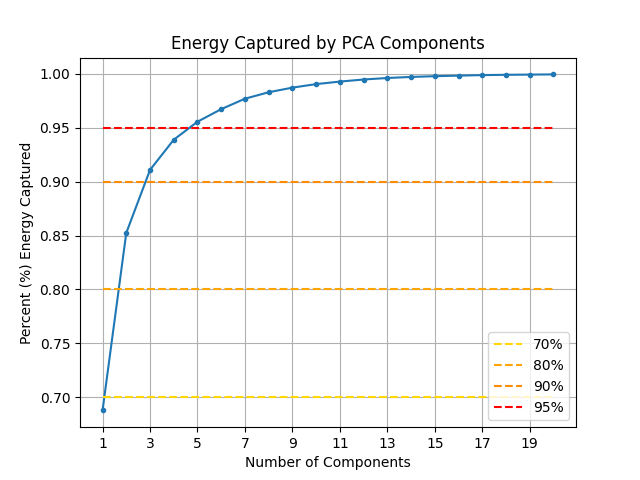
\includegraphics[width=.5\textwidth]{../visualizations/energy_by_components.png}
 	\caption{Visualizing each of the 3 slices including the location in our 3 dimensional average frequency object. We also visualize a slice which does not intersect the max frequency in order to convey how drastic the location of the max frequency is. In order to show this comparison things have been rescaled here.}\label{fig:f0}
\end{figure}

\begin{figure}[h]
    \centering
    \begin{subfigure}{0.4\textwidth}
        \centering
        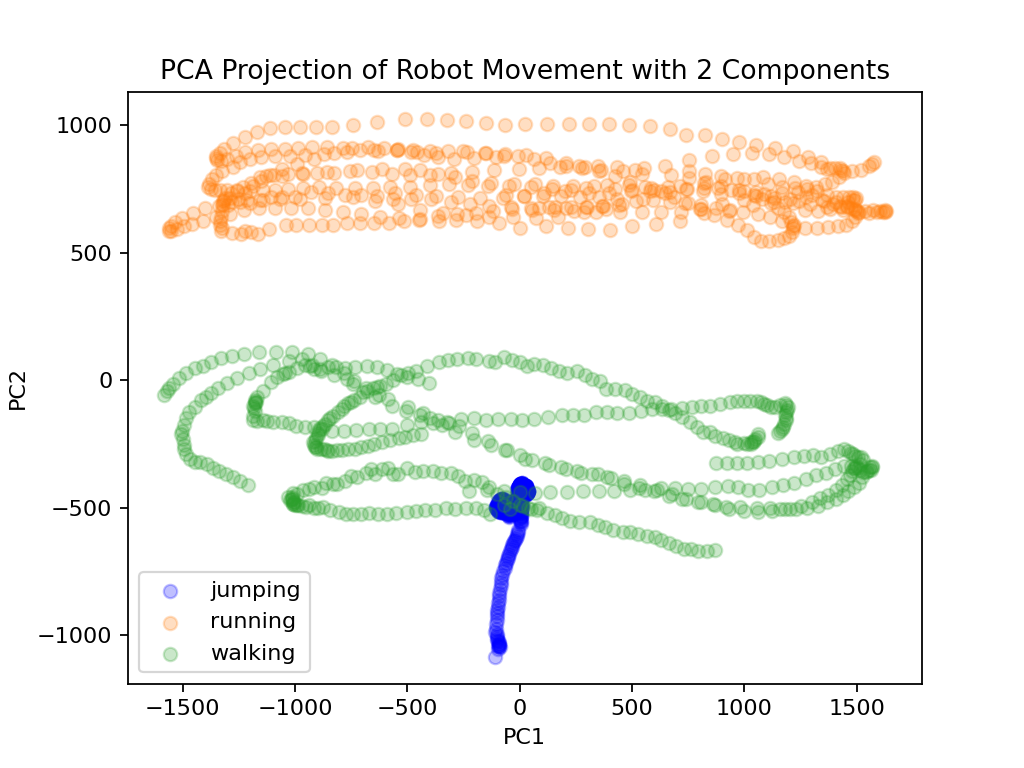
\includegraphics[width=\textwidth]{../visualizations/pca_2_components_plot.png}
        \caption{First image caption}
        \label{fig:image1}
    \end{subfigure}
    %\hspace{1mm}
    \begin{subfigure}{0.49\textwidth}
        \centering
        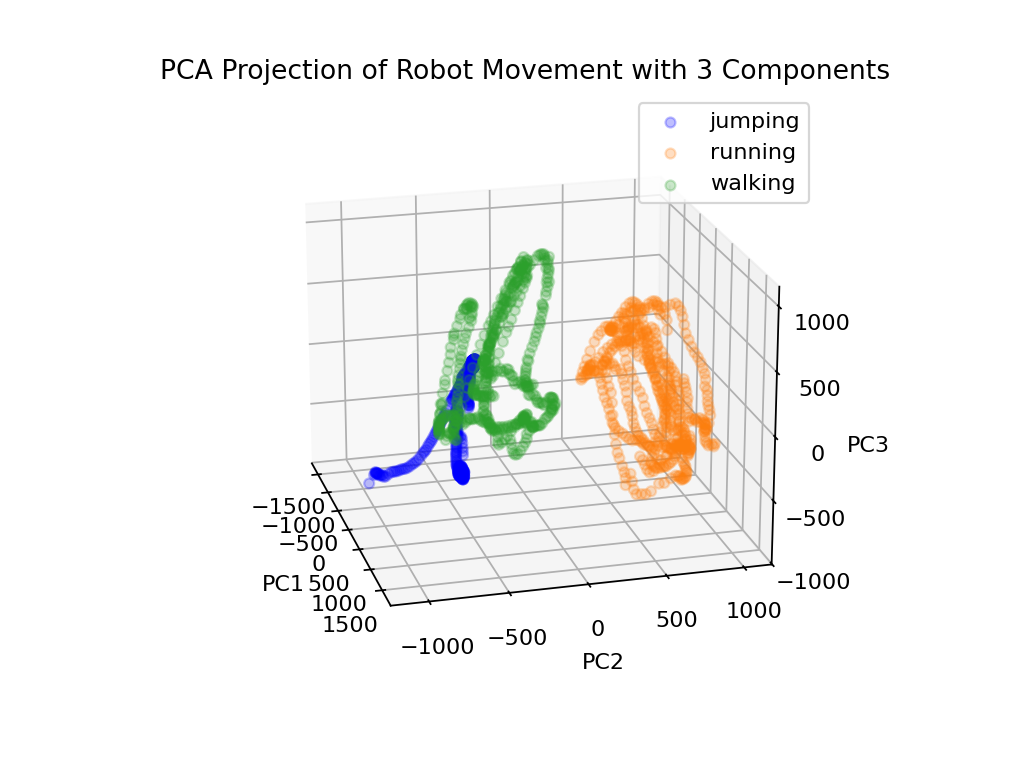
\includegraphics[width=\textwidth]{../visualizations/pca_3_components_plot.png}
        \caption{Second image caption}
        \label{fig:image2}
    \end{subfigure}
    \caption{Overall figure caption describing both images}
    \label{fig:f1}
\end{figure}


As seen in Figures \ref{fig:f0} and \ref{fig:f1}, then Figure \ref{fig:f2}.

\begin{figure}[h]
	\centering
	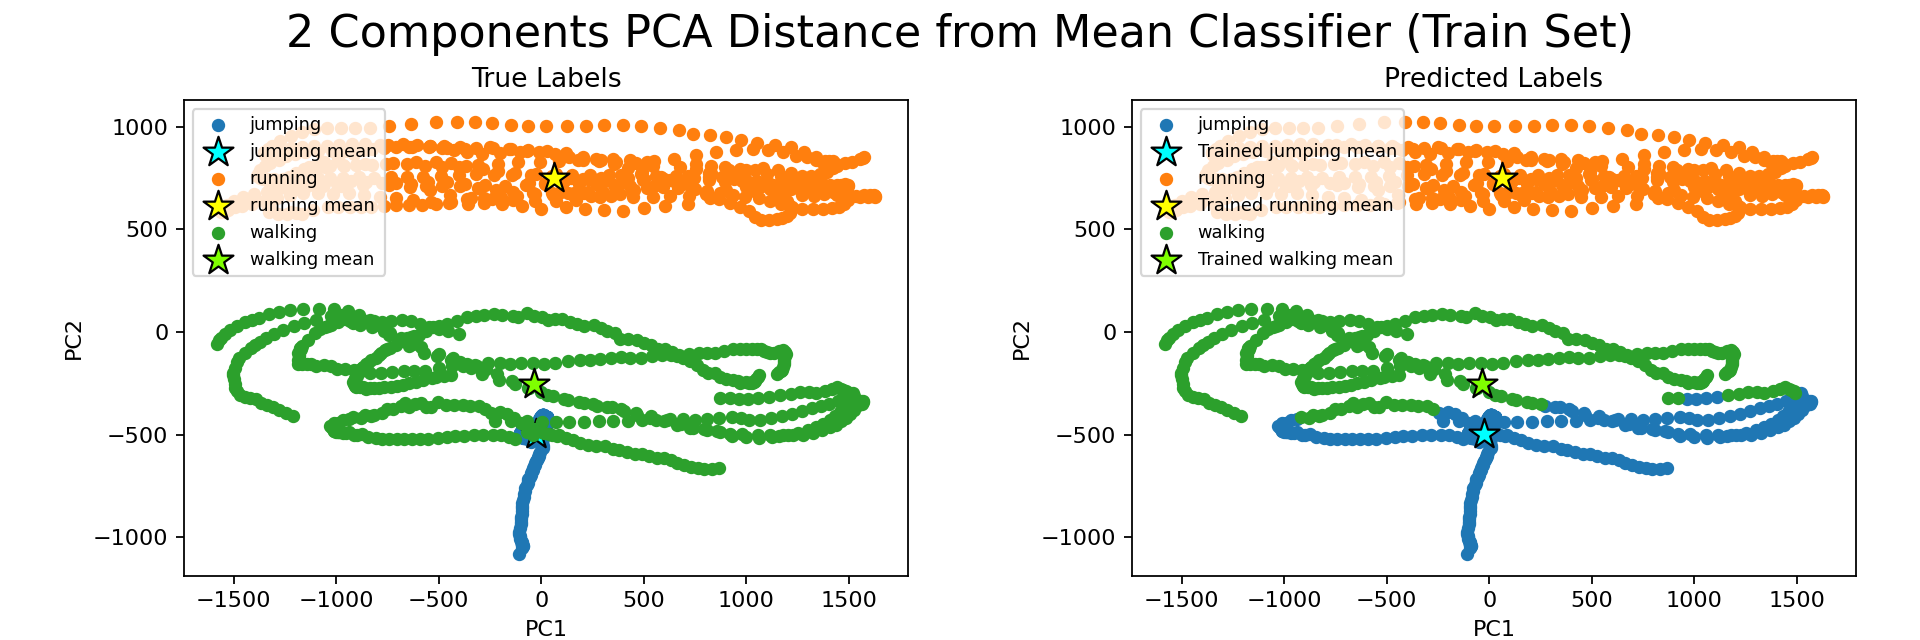
\includegraphics[width=.75\textwidth]{../visualizations/pca_distance_from_mean_classifier_2d.png}
 	\caption{The resulting path in 3 dimensions that we determined after applying Algorithms \ref{alg:dom_freq} and \ref{alg:filter}. In this iteration of the filter we used $\sigma=1.3$.}\label{fig:f2}
\end{figure}

\begin{figure}[h]
	\centering
	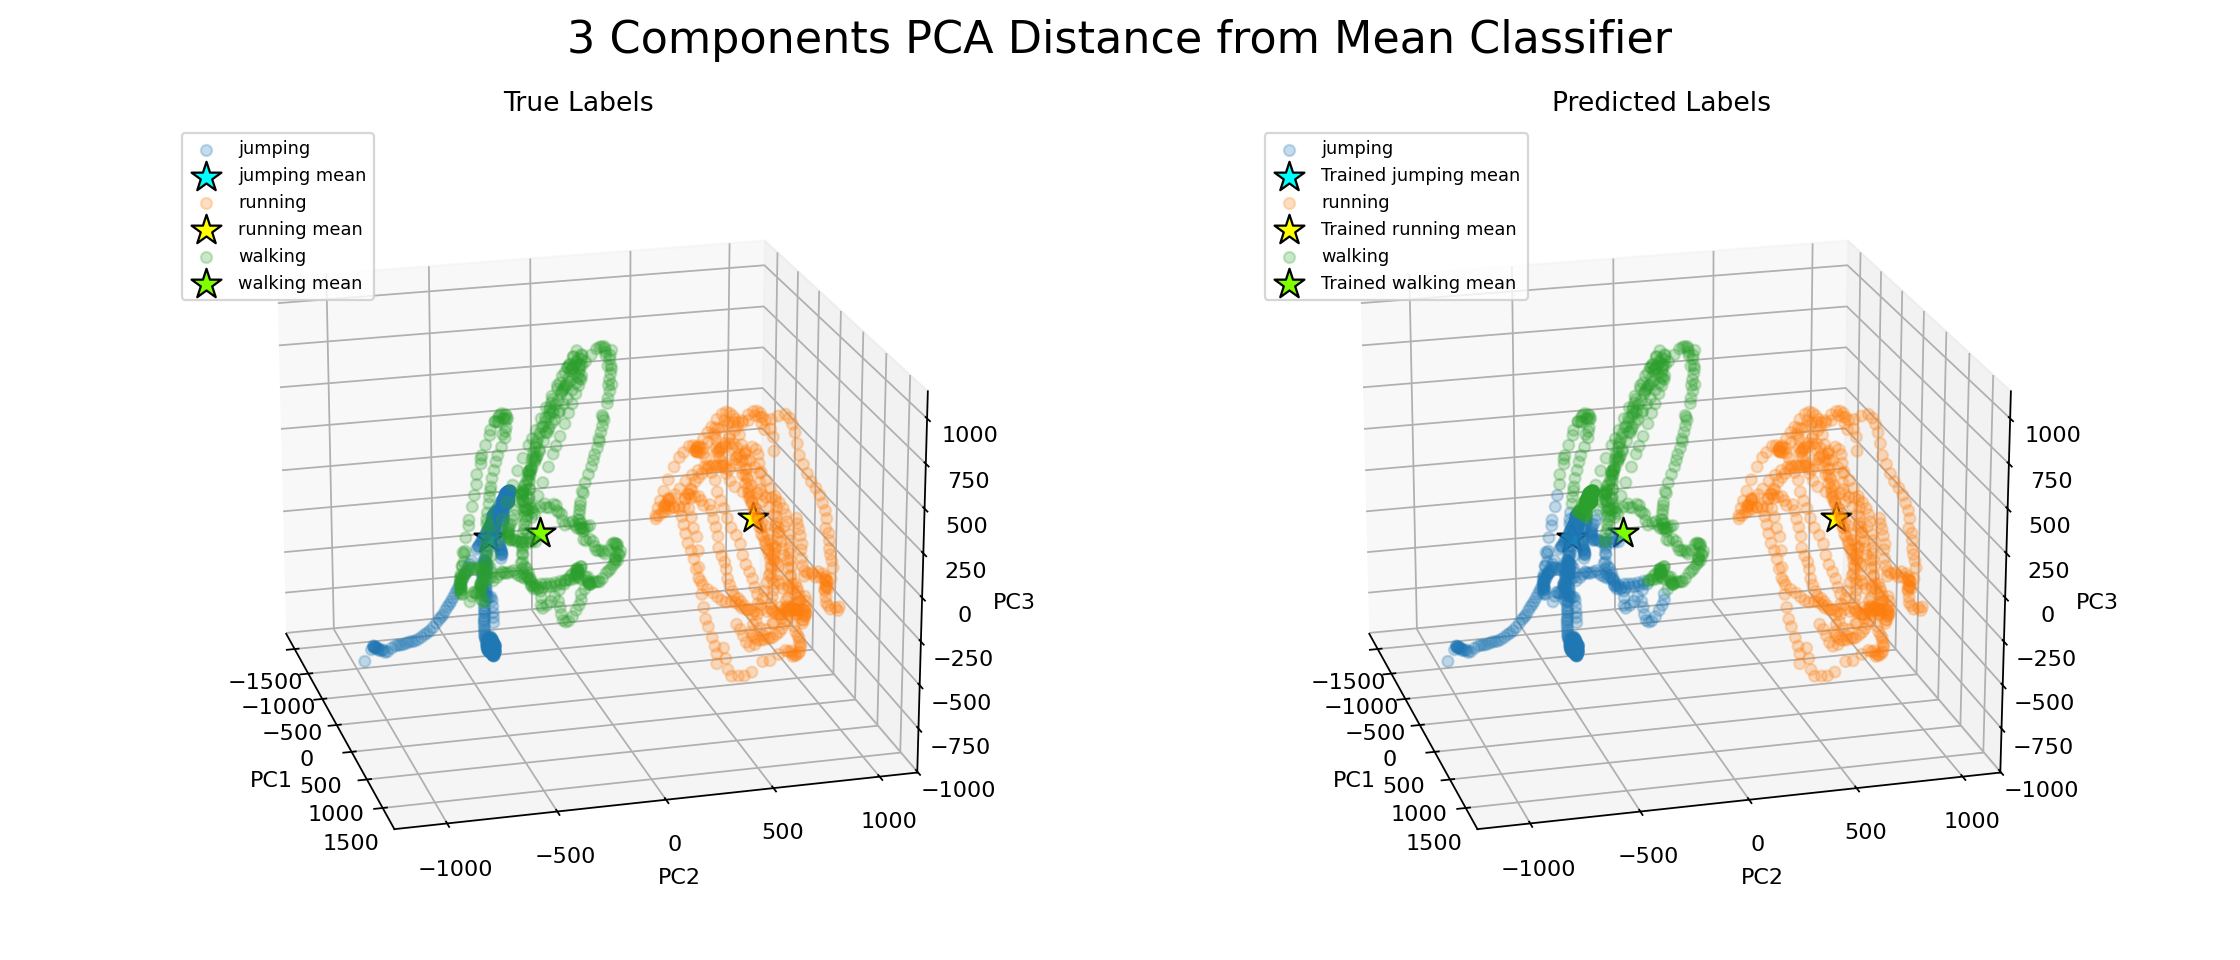
\includegraphics[width=.75\textwidth]{../visualizations/pca_distance_from_mean_classifier_3d.png}
 	\caption{This is just the 2 dimensional projection of the path given in the above 3d plot. The same value of $\sigma$ was used in the filter.}\label{fig:f3}
\end{figure}

\begin{figure}[h]
	\centering
	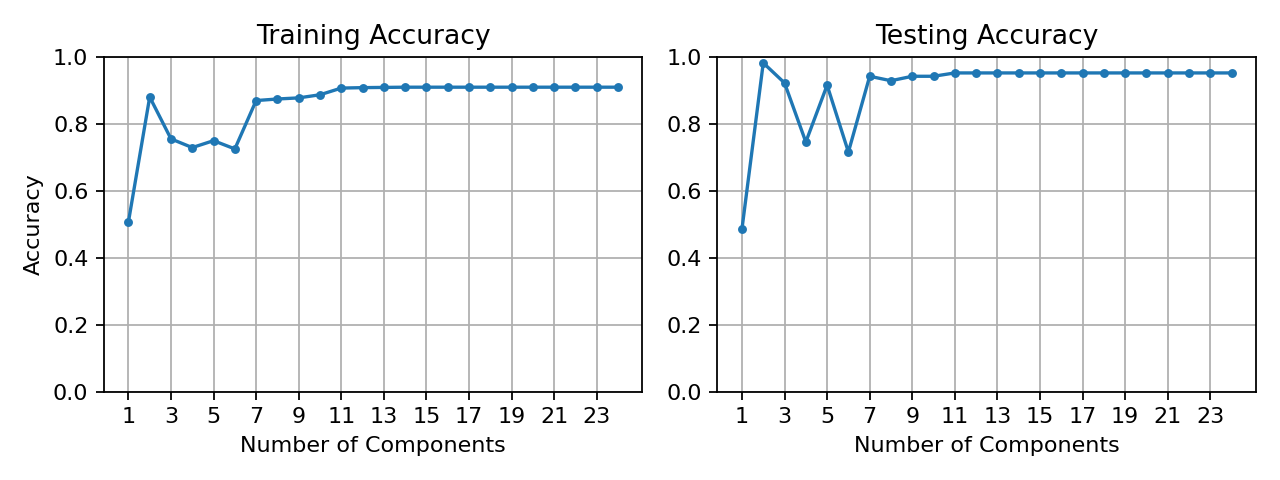
\includegraphics[width=.75\textwidth]{../visualizations/train_and_test_accuracy_by_num_components.png}
 	\caption{Visualizing each of the 3 slices including the location in our 3 dimensional average frequency object. We also visualize a slice which does not intersect the max frequency in order to convey how drastic the location of the max frequency is. In order to show this comparison things have been rescaled here.}\label{fig:f4}
\end{figure}

\begin{figure}[h]
	\centering
	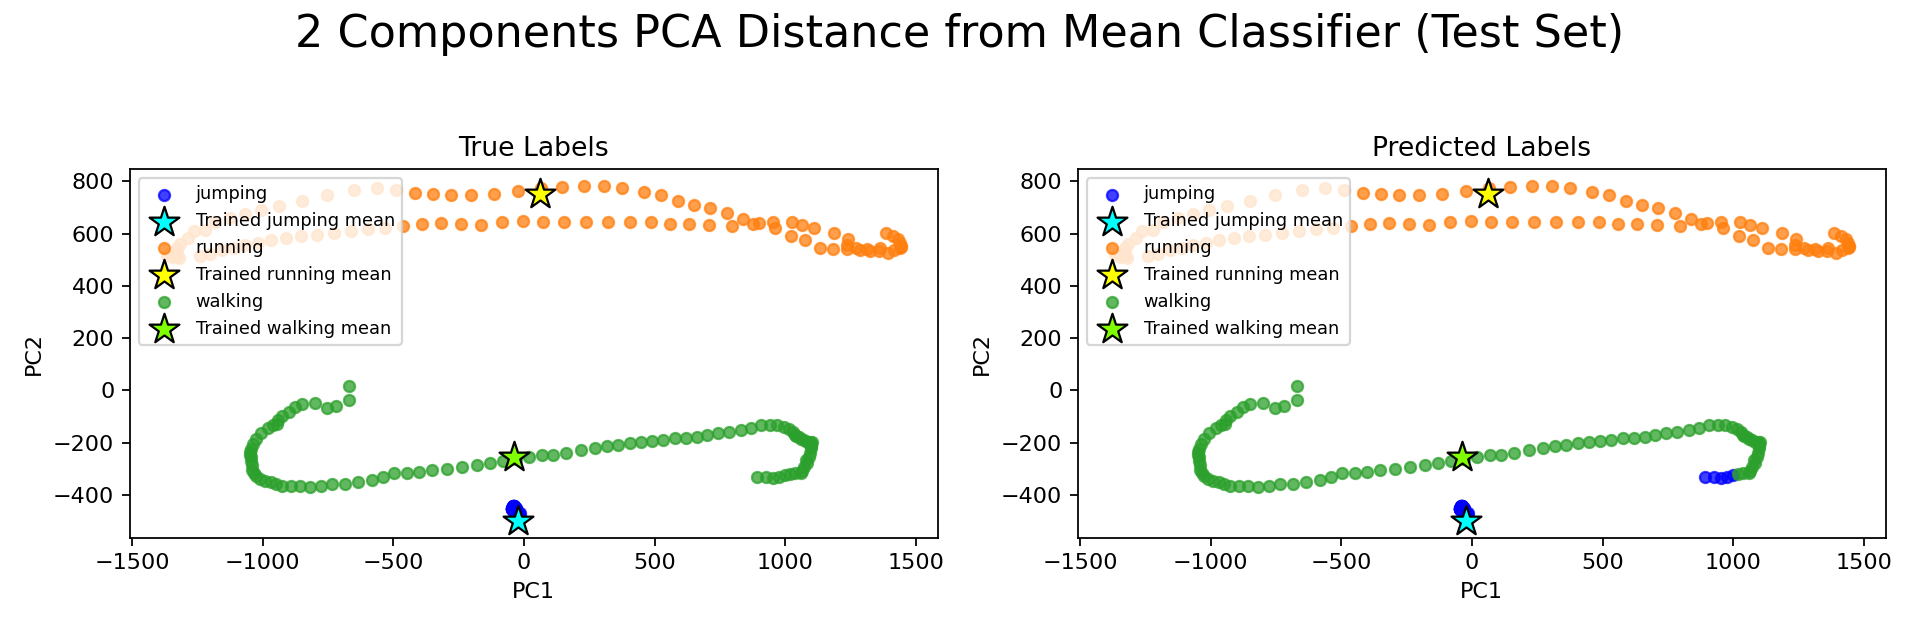
\includegraphics[width=.75\textwidth]{../visualizations/pca_distance_from_mean_classifier_2d_test_set.png}
 	\caption{Visualizing each of the 3 slices including the location in our 3 dimensional average frequency object. We also visualize a slice which does not intersect the max frequency in order to convey how drastic the location of the max frequency is. In order to show this comparison things have been rescaled here.}\label{fig:f5}
\end{figure}

\begin{figure}[h]
	\centering
	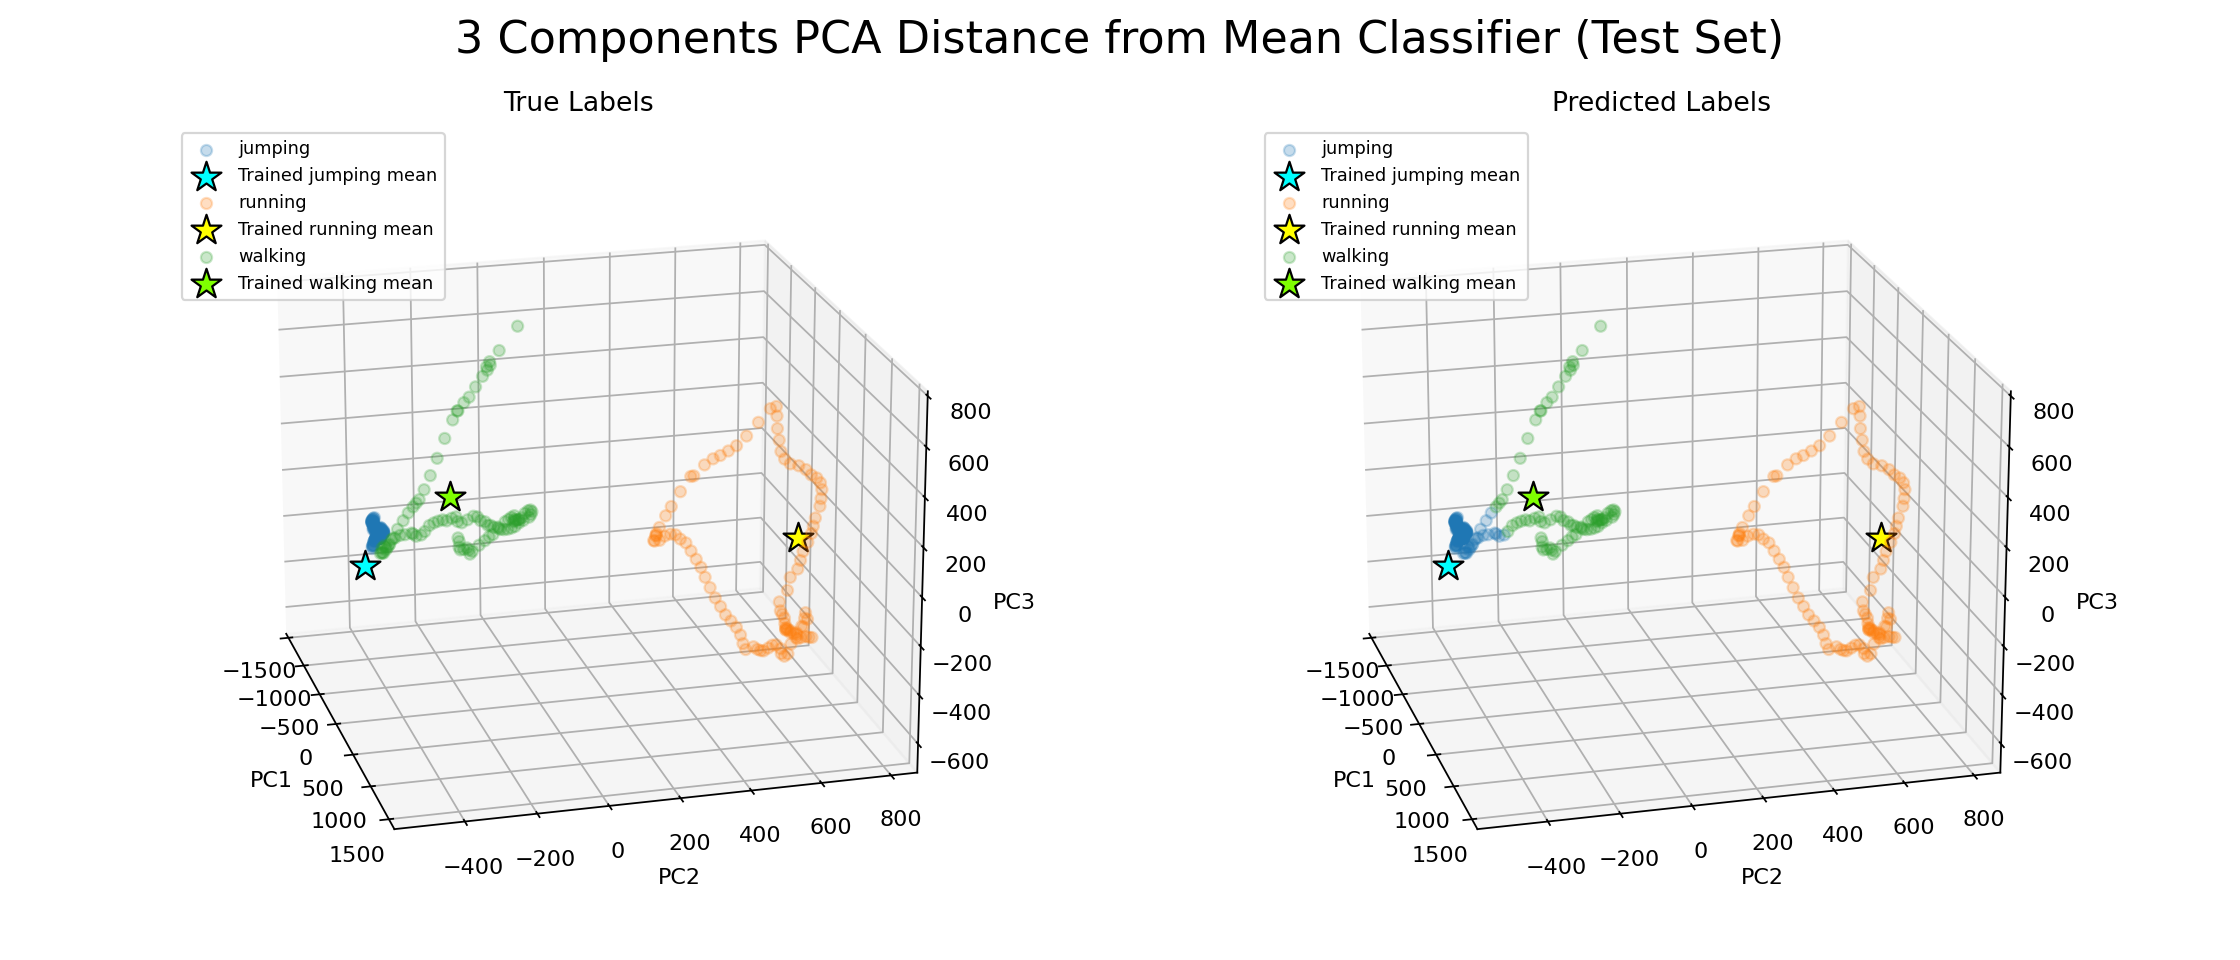
\includegraphics[width=.75\textwidth]{../visualizations/pca_distance_from_mean_classifier_3d_test_set.png}
 	\caption{Visualizing each of the 3 slices including the location in our 3 dimensional average frequency object. We also visualize a slice which does not intersect the max frequency in order to convey how drastic the location of the max frequency is. In order to show this comparison things have been rescaled here.}\label{fig:f6}
\end{figure}

\section{Summary and Conclusions}\label{sec:conclusions}
This is my summary and conc. \textbf{TODO:}

\section*{Acknowledgements} 

The author is thankful to Jaxon Tuggle for useful discussions about the process to find the correct dimensions to use when interpreting the training data samples we were given.
We would also like to thank Professor Eli Shlizerman for carefully instructing us in class.
Finally, it is necessary to thank the following students Nate Ward, Sophie Kamien, whose questions helped clarify understanding of the algorithm we implemented by giving chances to explain ideas and debug code together.

\bibliographystyle{abbrv}
\bibliography{references_hw2} % make sure this matches the .bib file for your corresponding document. You also have to maintain your references in the .bib file 

\end{document}
